\chapter{Dezvoltarea aplicațiilor}
\label{chapter:appdev}

\section{Introducere}
\label{sec:appdev:intro}

În momentul de față avem o varietate mare de dispozitive electronice cu care
interacționăm: de la sisteme complexe, cum ar fi calculatoarele personale sau
laptop-urile, la telefoanele mobile sau chiar ceasurile inteligente pe care le
folosim intens zilnic. Deși foarte diferite, toate aceste sisteme electronice au
un lucru în comun: toate rulează software.

Având în vedere marea varietate a sistemelor fizice pe care rulează aplicațiile
pe care le dezvoltăm, este foarte important să înțelegem toate aspectele
dezvoltării unui program și toate opțiunile pe care le avem la dispoziție în
acest proces. Astfel, putem face alegerile corecte pentru a dezvolta eficient o
aplicație adaptată dispozitivului fizic pe care va rula.

De exemplu, dacă dezvoltăm o aplicație ce va rula pe un ceas inteligent, trebuie
să ținem cont că avem resurse limitate comparativ la o aplicație ce va rula pe
un sistem desktop. În cazul unui ceas inteligent, avem mai puțină memorie și putere de
procesare și, mai mult, trebuie să ținem cont de consumul de energie pe care îl
are dispozitivul.

Alegerea unui limbaj potrivit pentru un program este esențială pentru succesul
acestuia. În funcție de tipul aplicației, trebuie ales limbajul adecvat având în
vedere proprietăți precum: viteza de execuție, ușurința de scriere a
codului, numărul de biblioteci existente, utilitarele existente, portabilitatea
și comunitatea din jurul limbajului.

\section{Limbaje de programare}
\label{sec:appdev:lang}

Un \textbf{limbaj de programare} definește un set de reguli folosite pentru a formula
instrucțiuni pe care calculatorul să le execute. Regulile limbajului constau în
cuvinte cheie, instrucțiuni care pot fi folosite și gramatica acestora, care se
mai numește și sintaxă.

Folosind un limbaj de programare, putem defini operații pe care dorim să le
executăm într-o anumite ordine. Acesta este practic programul pe care îl scriem.
Operațiile sunt rulate pe procesorul sistemului pe care dorim sa îl programăm,
dar înainte de a fi executate, ele trec printr-un proces de transformare.
Fiecare procesor cunoaște un anumit set de instrucțiuni pe care le poate
executa. Codul scris folosind aceste instrucțiuni se numește \textbf{cod mașină} și este
singurul limbaj pe care un procesor îl înțelege și îl execută. Prin urmare,
programul scris de noi într-un limbaj de programare este transformat în cod
mașină pentru a putea fi înțeles și executat.

La început, calculatoarele erau niște mașini cu capacitate de calcul mult mai
redusă, care puteau executa operații simple, în general stocate pe benzi
magnetice sau cartele perforate, ca în \labelindexref{Figura}{fig:appdev:card}. Odată cu evoluția procesoarelor și a mediilor de
stocare, a apărut limbajul de asamblare, folosit pentru a scrie programe mai
complexe. \textbf{Limbajul de asamblare} este un limbaj specific fiecărui procesor și are
în general o corespondență de aproximativ unu-la-unu între instrucțiunile de
asamblare și cele are procesorului. Practic, putem considera că fiecare
instrucțiune a limbajului de asamblare este tradusă printr-o altă instrucțiune a
procesorului. Codul sursă scris în limbaj de asamblare este transformat în cod
mașină de un asamblor.

\begin{figure}[!htbp]
	\centering
	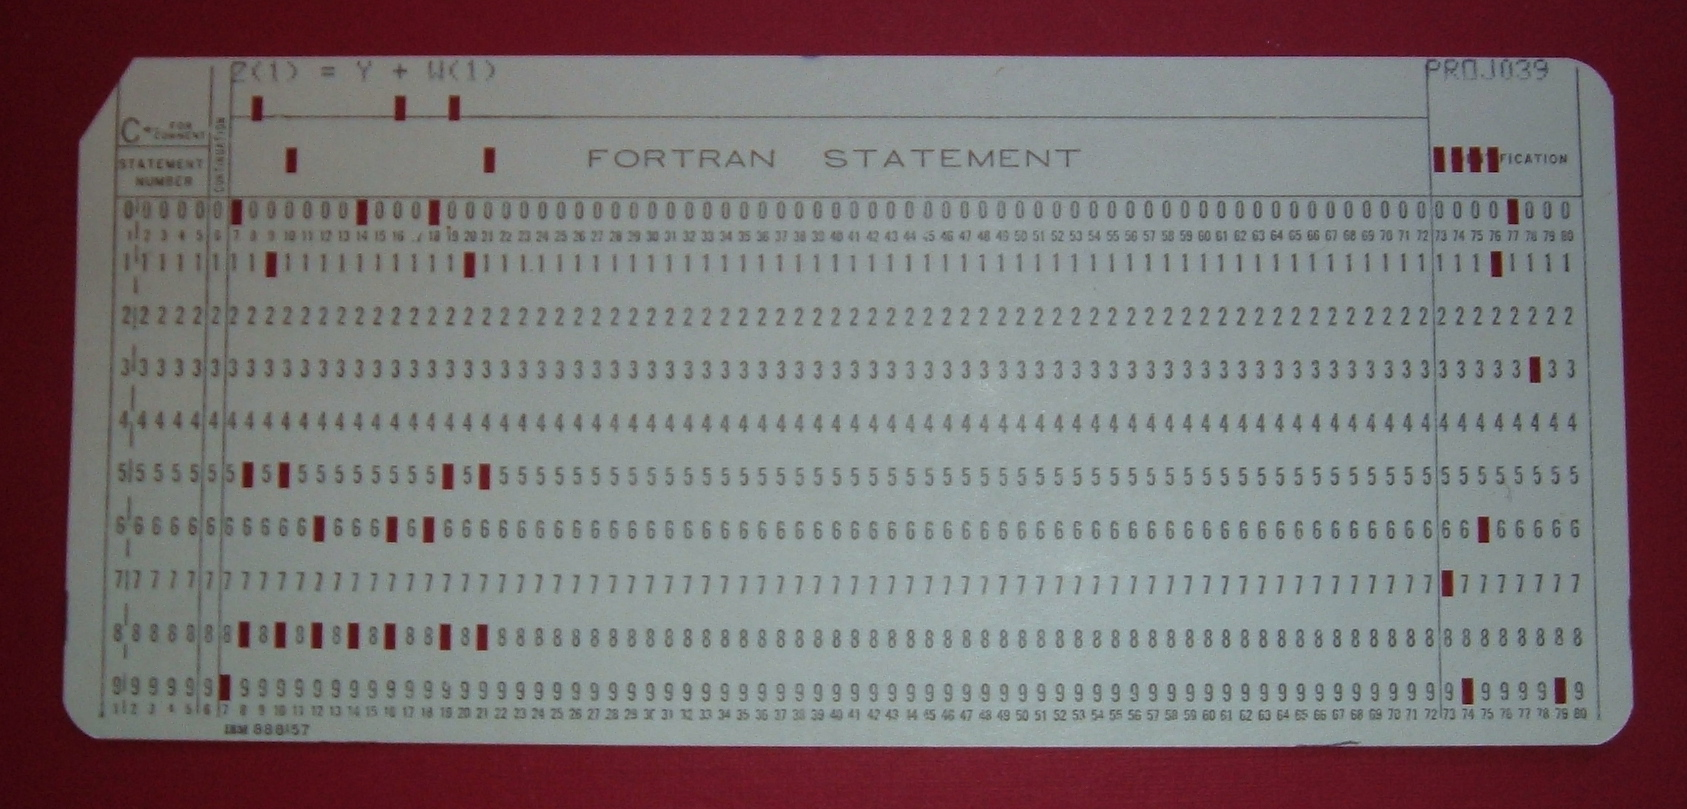
\includegraphics[width=15cm]{chapters/06-appdev/img/fortran-card-img.png}
	\caption{Program scris pe cartelă perforată\protect\footnotemark}
	\label{fig:appdev:card}
\end{figure}

\footnotetext{\url{https://en.wikipedia.org/wiki/Computer_programming_in_the_punched_card_era\#/media/File:FortranCardPROJ039.agr.jpg}
\textbf{CC BY-SA 2.5}}

În general, producătorul unui procesor definește și limbajul de asamblare
specific acestuia, pentru a oferi o variantă lizibilă a instrucțiunilor
procesorului. Scopul limbajului de asamblare a fost de a permite scrierea de
aplicații într-o manieră ușoară, la început acesta fiind singura modalitatea de
a dezvolta programe. Deși mai ușor de folosit decât codul binar, și limbajul de
asamblare este dificil de urmărit mai ales pentru programe lungi. De aceea, în
timp, au apărut limbajele mai complexe din punct de vedere al logicii, limbaje
ce folosesc comenzi apropiate ca structură de limbajul natural, și care sunt mai
ușor de urmărit. Acestea permit programatorilor să se concentreze pe logica
aplicației, nu pe limbajul efectiv și implementarea acestuia. Ele se numesc
\textbf{limbaje de nivel înalt}.

În prezent, majoritatea aplicațiilor sunt dezvoltate folosind limbaje de
programare de nivel înalt, care sunt mult mai ușor de “citit” de către
programatori. Totuși, pentru dezvoltarea de aplicații care controlează
dispozitive hardware și care trebuie să fie foarte eficiente în folosirea
resurselor (ex. drivere) se folosește uneori limbajul de asamblare, deși
cazurile acestea sunt destul de rare.

În mare parte, limbajele de programare folosite în zilele noastre sunt limbaje
de nivel înalt. Astfel, programatorii folosesc o sintaxă apropiată de limbajul
natural pentru dezvoltarea aplicațiilor, ceea ce ușurează întregul proces (se
folosesc cuvinte precum \textit{while}, \textit{if}, \textit{else}). Atunci
când scriem un program, totul pornește de la ideea clară a ce vrem să obținem
prin acel program. Mai exact, trebuie să stabilim clar ce vrem să facă
programul. După aceea, următorul pas este să structurăm ideea și să o
\textit{traducem} în limbajul de programare folosit. Așa obținem programul final
ce apoi poate fi rulat, proces sumarizat în \labelindexref{Figura}{fig:appdev:idea-to-program}.

\begin{figure}[htbp]
	\centering
	\def\svgwidth{\columnwidth}
	\includesvg{chapters/06-appdev/img/lang-idea.svg}
        \caption{De la idee la program}
	\label{fig:appdev:idea-to-program}
\end{figure}

Fișierele pe care programatorii le scriu se numesc \textbf{fișiere cod sursă}, ele conțin
practic instrucțiuni scrise într-un anume limbaj de programare, de cele mai
multe ori, limbaj de nivel înalt. Codul sursă scris astfel nu poate fi executat
pentru că procesorul nu îl înțelege. Cum am menționat deja, procesorul înțelege
doar codul mașină. Drept urmare, pentru a executa programul, e necesar să
transformăm codul sursă în cod mașină.

Procesul de transformare a codului sursă în cod mașină se numește \textbf{compilare}.

Bazat pe modul în care codul de nivel înalt este transformat și rulat pe
procesor, putem clasifica limbajele de programare în limbaje compilate sau
interpretate. Diferența între cele două este că pentru a rula un limbaj
compilat, acesta este întâi transformat în cod mașină, rezultând un fișier
executabil, care apoi poate fi rulat oricând. Pe de altă parte, un limbaj
interpretat este executat direct, prin intermediul unui interpretor.
Interpretorul este cel care ia fiecare instrucțiune, o transformă în cod mașină
iar aceasta este executată imediat.

Fiecare dintre cele două tipuri de a rula cod sursă, compilare sau interpretare,
are avantaje și dezavantaje de care este important să ținem cont când alegem
limbajul de programare pentru dezvoltarea unei aplicații.

Principalul avantaj al unui limbaj compilat este viteza de execuție. Odată
generat fișierul executabil, acesta va fi rulat de către procesor de oricâte ori
dorim, astfel compilarea este un proces separat de execuția programului și are
loc o singură dată. În schimb, în cazul unui limbaj interpretat, la fiecare
rulare, codul sursă va fi interpretat linie cu linie de către
interpretor, acesta fiind de fapt cel care execută acțiunile programului, proces
care e mai lent.

Unele interpretoare mai eficiente vor încerca sa compileze parțial codul sursă
și să îl execute direct pe procesor. Practic, în acest caz, codul sursă se
compilează la fiecare rulare.

Pe de altă parte, un limbaj interpretat are mai multă portabilitate. Cum am
precizat deja, codul mașină rezultat în urma compilării poate rula doar pe un
anumit tip de procesor. Deci pentru a rula aceeași aplicație pe arhitecturi
(procesoare) diferite, avem nevoie de un fișier executabil pentru fiecare tip de
arhitectură. În aceea ce privește limbajele interpretate, putem folosi aceleași
fișiere care sunt transformate de către interpretor în codul mașină specific
procesorului.

Majoritatea limbajelor de programare apărute în ultima perioadă sunt considerate
limbaje hibride. Ele îmbină elemente ale ambelor procese, compilare și
interpretare, pentru a obține atât portabilitate, cât și viteză în execuție.

Este important de reținut că indiferent de limbaj (compilat, interpretat sau
hibrid), procesorul știe să ruleze doar cod mașină, așa că orice cod sursă va fi
la un moment dat transformat în cod mașină, iar pentru programatori este
important dacă limbajul folosit este unul compilat, interpretat sau hibrid. Este
important să cunoaștem tipul unui limbaj de programare și avantaje și
dezavantaje sale pentru a putea alege în funcție de nevoile pe care le avem.

De exemplu, dacă ne dorim să dezvoltăm un joc tip curse de mașini, avem nevoie
de rapiditate în execuție, față de o aplicație de organizare a lucrului în
echipă, unde ne dorim să putem acoperi cât mai multe platforme.

\section{Limbaje compilate}
\label{sec:appdev:compiled-lang}

Limbajele compilate sunt cele unde codul sursă este transformat în fișiere
executabile, ce sunt apoi rulate pe procesor, în urma unui proces care se
numește compilare. Astfel, instrucțiunile specifice limbajului de programare
sunt transformate de compilator în instrucțiuni pe care procesorul le înțelege.

În procesul de compilare codul sursă este prelucrat și trece prin mai multe
etape intermediare ca în \labelindexref{Figura}{fig:appdev:compile-phases}.

\begin{enumerate}
	\item compilare: codul sursă este transformat în cod în limbaj de
		asamblare
	\item asamblare: codul în limbaj de asamblare este transformat în cod
		mașină;
        \item link-editare (sau linking): se fac legăturile către fișiere externe care conțin
		simboluri sau funcții apelate din fișierul sursă; dacă avem o
		funcție definită într-un fișier și folosită în altul,
		implementarea funcției trebuie legată de apelul ei.
\end{enumerate}

\begin{figure}[htbp]
  \centering
  \def\svgwidth{0.6\columnwidth}
  \includesvg{chapters/06-appdev/img/comp-steps.svg}
  \caption{Etapele compilării}
  \label{fig:appdev:compile-phases}
\end{figure}

În teorie, pentru fiecare limbaj de programare ar trebui să existe un compilator
care să cunoască gramatica specifică acestuia, instrucțiunile
specifice unui procesor și care să facă transformarea din cod sursă în cod
mașină.

Pentru că există un număr foarte mare de limbaje și un număr mare de procesoare
diferite, în practică, nu avem cate un compilator diferit. În general, există
framework-uri de compilator care au suport pentru mai multe limbaje de programare (de exemplu C sau C++ sau D), respectiv alte
componente care au suport pentru mai multe arhitecturi de procesor (de exemplu x86 sau ARM sau MIPS). Astfel, un compilator poate genera cod pentru diferite arhitecturi pornind de la diferite tipuri de limbaje. În general aceste compilatoare au un limbaj intern, numit limbaj intermediar care facilitează aceste traduceri din limbaj în cod mașină de procesor, așa cum este indicat în \labelindexref{Figura}{fig:appdev:intermediary}.

\begin{figure}[htbp]
  \centering
  \def\svgwidth{0.6\columnwidth}
  \includesvg{chapters/06-appdev/img/comp-backend-frontend.svg}
  \caption{Traducerea în limbaj intermediar}
  \label{fig:appdev:intermediary}
\end{figure}

\subsection{Exemple de limbaje de programare compilate}
\label{sec:appdev:compiled-lang:ex}

Deși am prezentat avantajele și dezavantajele folosirii unui limbaj de
programare compilat, dacă alegem că aceasta este opțiunea potrivită, avem un
număr mare de limbaje compilate din care putem alege. În continuare vom descrie
câteva din cele mai folosite și particularitățile de care trebuie să ținem cont
în luarea unei decizii.

\subsubsection{C}
\label{sec:appdev:compiled-lang:c}

C este un limbaj de programare care a fost dezvoltat în anii 1970 pentru a fi
folosit la implementarea sistemului de operare Unix. Până la apariția limbajului
C, sistemele de operare erau scrise în limbaj de asamblare. C aduce un nivel de
abstractizare peste limbajul de asamblare, care ușurează scrierea programelor.

Pentru că limbajul permite accesarea ușoară a resurselor hardware, aplicațiile
dezvoltate în C prezintă un risc mai mare de securitate, dacă acestea nu sunt implementate cu
atenție. Din aceleași considerente și probabilitatea de a genera erori în timpul
implementării este mai mare. În plus, C are un nivel de abstractizare foarte
redus, adică nu avem la dispoziție funcții care să execute operații complexe, de
aceea nu este un limbaj folosit pentru prototipare. Este recomandat să folosim C
dacă stăpânim bine limbajul și nu riscăm să generăm erori și dacă ne dorim o
aplicație care să consume cât mai puține resurse.

Preponderent, limbajul C este folosit pentru a dezvolta sisteme de operare și
drivere pentru acestea.

\subsubsection{C++}
\label{sec:appdev:compiled-lang:cpp}

C++ este un limbaj de programare de nivel înalt gândit pentru dezvoltarea de
aplicații. Este o adaptare a limbajului C pentru a-l face mai ușor de folosit.
În comparație cu alte limbaje mai noi, C++ este un limbaj mai complex și mai dificil de
utilizat. Totuși, un număr mare de aplicații existente axate pe performanță sunt implementate folosind C++.

\subsection{Pascal}
\label{sec:appdev:compiled-lang:pascal}

Pascal a fost dezvoltat în anii 1960, având ca scop principal dezvoltarea de
programe pentru descrierea de algoritmi. Limbajul a fost gândit pentru educație,
pentru a fi utilizat în predarea algoritmilor.

Deși nu este un limbaj pe care să îl luam în calcul în dezvoltarea aplicațiilor,
pentru că există alte limbaje mai moderne, poate fi în continuare luat în calcul
în scopuri didactice.

\subsection{Alte limbaje}
\label{sec:appdev:compiled-lang:other}

Alte limbaje compilate sunt D, Go (folosit pentru scrierea sistemului de
containere Docker) și Rust (folosit de Firefox pentru Servo, motorul de randare
a paginilor web)

\section{Limbaje interpretate}
\label{sec:appdev-langs-int}

Limbajele interpretate sunt cele care sunt transformate în cod mașină în timpul
execuției.

Pentru a putea rula o aplicație dezvoltată într-un limbaj de programare
interpretat, avem nevoie de un program care ia fiecare linie din codul sursă și
o transformă în cod mașină. Acest program se numește interpretor.

Diferența între o aplicație compilată și una interpretată este că spre deosebire
de compilator, care generează un întreg fișier executabil care poate fi apoi
rulat, interpretorul ia fiecare linie, generează codul mașină aferent ei, codul
este rulat pe procesor, după care operația este reluată. Deși acest proces
crește timpul de execuție al aplicației, sunt avantaje pe care limbajele
interpretate le au față de cele compilate.

În primul rând, programele scrise în astfel de limbaje pot fi direct rulate pe
orice arhitectură, atâta timp cât există un interpretor instalat. Acest lucru înseamnă
că putem copia codul sursă de pe un sistem care rulează Windows pe unul care
rulează macOS. În plus, pentru că toate instrucțiunile trec prin interpretor,
limbajele interpretate nu oferă acces direct la resursele hardware, ceea ce le
face mai sigure, dar și mai ineficiente. De aceea astfel de limbaje sunt
recomande pentru dezvoltarea de aplicații care nu țin de sistemul de operare.

Pe de altă parte, limbajele interpretate presupun ca orice mașină care va rula
aplicația dezvoltată, trebuie să conțină codul sursă ce va fi rulat. Sunt cazuri
în care nu se dorește publicarea codului sursă ar fi de preferat un limbaj
compilat, care permite distribuirea unui executabil.

\subsection{Exemple de limbaje de programare interpretate}
\label{sec:appdev:interpreted-lang:ex}

În prezent utilizarea limbaje de programare pur interpretate este în scădere.
Acestea au ajuns să fie înlocuite de alte limbaje de programare, majoritatea
hibride. Totuși, dacă vom ajunge să lucrăm la aplicații complexe dezvoltate cu
ani în urmă, există posibilitatea să ajungem să scriem cod sursă în limbaje
precum PHP sau Perl.

PHP este un limbaj folosit preponderent pentru dezvoltarea de servere web. Mai
nou este înlocuit de Node.js, dar încă mai putem găsi aplicații web dezvoltate
în PHP.

Perl e un alt limbaj interpretat folosit pentru dezvoltare web. Este considerat
predecesorul PHP, deci este tot mai rar întâlnit.

\section{Limbaje hibride}
\label{sec:appdev:hybrid-lang}

Limbajele de programare hibride îmbină elemente de compilare cu elemente de
interpretare, pentru a rezulta în aplicații portabile, rapide și sigure.

Pentru că principalul dezavantaj al programelor interpretate este timpul mare de
execuție, una din îmbunătățirile aduse interpretoarelor este posibilitatea de a
transforma codul sursă într-un cod intermediar, care se numește \textbf{bytecode}, care
va fi apoi interpretat. Bytecode-ul este practic codul mașină al
interpretorului, deci transformarea acestuia în cod mașină este mult mai rapidă.
Practic, la rularea unui program, este generat un fișier intermediar care
conține bytecode, iar interpretorul ia apoi instrucțiuni din bytecode și le
transformă în cod mașină. Putem deci considera că avem două etape în procesul de
rulare: compilare către bytecode și apoi interpretare.

Pentru că în acest caz interpretorul are propriul limbaj mașină, acesta nu cunoaște
un limbaj de programare anume, ci el transformă bytecode-ul specific în cod
mașină, interpretorul se mai numește și \textbf{mașină virtuală} (ex. Java Virtual
Machine). Un avantaj pe care mașina virtuală îl aduce este posibilitatea de a
genera bytecode-ul și de a distribui fișiere bytecode în locul codului sursă.
Astfel codul sursă al aplicației nu este făcut public odată cu distribuția
aplicației.

Odată generat bytecode-ul, acesta poate fi transformat în cod mașină în două
moduri diferite. Fie se ia tot bytecode-ul și se transformă în cod mașină, după
care codul mașină este executat (compilare \textit{ahead-of-time}, sau JIT\abbrev{JIT}{just-in-time}), fie se iau bucăți din
bytecode și se transformă în cod mașină în timpul rulării (compilare
\textit{just-in-time}).

Compilarea \textit{ahead-of-time} funcționează ca procesul normal de compilare, doar că
se transformă bytecode în cod mașină. Odată generat codul mașină acesta este
executat. Avantajul acestei metode este timpul rapid de execuție. În schimb,
timpul de pornire a aplicației crește (timpul necesar pentru a transforma
bytecode în cod mașină).

Compilarea \textit{just-in-time} (JIT) presupune ca bucăți de cod care urmează să fie executate
să fie transformate în cod mașină în timpul rulării. Interpretorul analizează
blocul de cod care urmează să fie executat și îl transformă în cod mașină.

În plus, interpretorul are anumite mecanisme care îi permit să țină cont de
factori precum frecvența de execuție a unui anumit bloc de cod și eficientizează
procesul prin stocarea în memorie a codului mașină, pentru a nu transforma
același cod de mai multe ori, deci făcând procesul și mai eficient. Totuși, spre
deosebire de compilarea ahead-of-time, JIT are un
timp de execuție mai mare, dar timpul de pornire al aplicației scade.

\subsection{Exemple de limbaje de programare hibride}
\label{sec:appdev:hybrid-lang:ex}

În general, limbajele pe care le întâlnim cel mai frecvent astăzi sunt limbaje
hibride, precum Java, Python sau JavaScript. Cum multe din aplicațiile pe care
le folosim zi de zi au devenit aplicații web, limbajele orientate spre așa ceva
au crescut în popularitate.

\subsubsection{Java}
\label{sec:appdev:hybrid-lang:java}

Java este un limbaj de programare folosit pentru dezvoltarea de aplicații
enterprise care a fost dezvoltat de Sun Microsystems. Oracle a cumpărat Sun
Microsystems, așa că astăzi Java este întreținut de către Oracle. Paradigma pe
care se bazează Java este programarea orientată pe obiecte. Acesta facilitează
scrierea unui cod cât mai modularizat și refolosibil.

Idee de bază care a stat la baza limbajului Java a fost portabilitatea. Se dorea
scrierea unui program o singură dată și rularea lui pe multe platforme diferite
fără a face vreo modificare și fără a fi necesară distribuirea sursei. Inițial a
fost folosit în programe de navigare sub forma de \textit{Java Applets}, mici
aplicații scrie care se putea include într-o pagină.

Fiind destinat dezvoltării de aplicații pentru companii, platforma Java este are
două componente, compilatorul care generează bytecode-ul (Java Development Kit -
JDK \abbrev{JDK}{Java Development Kit}) și mașina care rulează bytecode-ul (Java
Runtime Environment - JRE \abbrev{JRE}{Java Runtime Environment}). Astfel pentru
distribuția aplicației nu este necesară distribuția codului sursă.

\subsubsection{C\#}
\label{sec:appdev:hybrid-lang:csharp}

C\# este un limbaj de programare similar cu Java, dezvoltat de Microsoft. Este
principalul limbaj de dezvoltare pentru platforma Windows, fiind integrat
inclusiv în motoare de jocuri (de exemplu Unity).

\subsubsection{Python}
\label{sec:appdev:hybrid-lang:python}

Python este un limbaj dezvoltat inițial cu scopul de a fi folosit pentru a
învăța programare, principalul avantaj fiind ca oferă o lizibilitatea mare
codului. A devenit foarte cunoscut datorită unor proiecte precum GNOME (inițial)
și OpenStack, precum și datorita bibliotecilor de matematică avansate.

Python este folosit pentru automatizarea administrării sistemului, prin
scripturi simple. Este de asemenea foarte folosit în educație, codul sursă fiind
ușor de urmărit. În plus, Python impune reguli de indentare, ceea ce îl face
potrivit ca prim limbaj de programare care obișnuiește elevii cu necesitatea de
a indenta codul. Limbajul mai este folosit în cercetare, find o variantă mai
,,ușoară'' față de alte limbaje științifice cum ar fi Matlab, R sau Julia.

O altă utilizare a limbajului Python este pentru dezvoltarea de servere web, cu
ajutorul bibliotecilor Flask și Django.

\subsubsection{JavaScript}
\label{sec:appdev:hybrid-lang:js}

JavaScript este un limbaj folosit pentru dezvoltarea de aplicații web. Are o
sintaxa similară cu limbajele C și Java. Deși se numește JavaScript, în afară de
sintaxa similară, nu are nimic în comun cu Java.

La început JavaScript a fost folosit pentru partea de interfață a aplicațiilor
web, interpretorul de JavaScript fiind integrat în browsere. Odată cu apariția
platformei Node.js, aplicațiile JavaScript pot fi rulate și în afara
browserului. Astfel, JavaScript este folosit pentru aplicații simple, pentru
automatizarea operațiilor, dar mai ales pentru dezvoltarea de servere web, prin
intermediul bibliotecii Express.

În principiu, dacă ne dorim să dezvoltăm o aplicație web, JavaScript, împreună
cu Node.js sunt o opțiune importantă de luat în calcul.

\section{Dezvoltarea unui program}
\label{sec:appdev:dev}

Până acum am discutat despre limbajele de programare uzuale și cum acestea se
diferențiază între ele și despre cum codul sursă pe care noi îl scriem rulează
pe procesor. Întrebarea pe care urmează să o punem este: \textit{ce presupune
dezvoltarea unui program}?

\subsection{Scrierea codului sursă}
\label{sec:appdev:dev-stages:write}

În primul rând, dezvoltarea unui program constă în scrierea efectivă a codului
sursă; practic, acest pas se rezumă la a crea fișiere text și a le edita. De
aceea, aplicația principală de care avem nevoie în dezvoltarea unui program este
un \textbf{editor de text}.

În ceea ce privește editoarele de text, avem un număr mare de editoare diferite
din care putem alege, pornind de la unele foarte simple care au ca scop editarea
unui fișier text, la aplicații complexe adaptate dezvoltării de programe. În mod
normal, orice editor poate fi folosit pentru scrierea de cod, chiar și Notepad
din Microsoft Windows, totuși este de preferat să folosim unul adaptat scrierii
de cod, pentru a ne ușura munca.

Editoarele adaptate dezvoltării de programe vin cu anumite caracteristici care
ne ajută în procesul de dezvoltare cum ar fi indentarea automată a codului, evidențierea cuvintelor cheie, numerotarea liniilor, gruparea secvențelor de cod.

Ținând cont de numărul mare de limbaje de programare existente, fiecare cu
particularitățile sale, este imposibil ca un editor să cuprindă toate aspectele
fiecărui limbaj. De aceea, majoritatea acestor editoare permit instalarea de
extensii care aduc funcționalități în plus sau aduc funcționalități specifice
pentru un anumit limbaj.

În continuare vom descrie cele mai cunoscute editoare folosite pentru scrierea
programelor.

\subsection{Editoare în mod text}
\label{sec:appdev:dev-stages:editor}

\subsubsection{Vim}
\label{sec:appdev:dev-stages:editor:vim}

Vim este un editor care funcționează în linie de comandă, fiind versiunea
îmbunătățită a vi, editor care se găsește pe toate sistemele Unix. Este un editor foarte configurabil, dar nu foarte ușor de
folosit pentru începători. Acest lucru este datorat lipsei interfeței grafice,
tot meniul fiind transpus prin comenzi. Deși pentru utilizatorii experimentați
acest lucru poate reprezenta un avantaj aducând rapiditate în folosire, pentru
începători, lipsa cursorului și necesitatea de a memora comenzi îngreunează
folosirea editorului.

Chiar dacă există multe variante de editoare mai intuitive, vă recomandam
familiarizarea cu Vim, sau chiar cu varianta redusă, vi, tocmai pentru că este
unul din puținele editoare disponibile pe orice sistem Unix.

Pentru familiarizarea cu Vim și comenzile de bază, recomandăm parcurgerea
tutorialului \cmd{vimtutor}. Este suficient să rulați comanda \cmd{vimtutor} în terminal și
tutorialul va începe.

Deși putem găsi vi pe orice sistem Unix, doar unele distribuții vin cu editorul
vim instalat. Pentru a instala Vim pe sistemele Debian/Ubuntu, rulăm comanda \cmd{sudo apt
install vim}.

\subsubsection{Alte editoare}
\label{sec:appdev:dev:editor:other}

Alte editoare similare cu Vim, care funcționează tot în linie de comandă, sunt
Nano, Pico și Emacs. La fel ca Vim, este se găsesc frecvent pe sistemele Unix, sunt
folosite la editarea rapidă, cum ar fi editarea unor fișiere de configurare.

\subsection{Editoare în interfață grafică}
\label{sec:appdev:dev:editor-gui}

\subsubsection{Sublime Text}
\label{sec:appdev:dev:editor-gui:sublime}

Sublime Text este un editor de cod avansat. Permite crearea sau editarea
facilă a unor programe complexe, alcătuite din mai multe fișiere. Pe lângă
posibilitatea de a edita structura de fișiere și directoare a proiectului,
editorul recunoaște limbajele de programare cele mai folosite și evidențiază
cuvintele cheie specifice fiecărui limbaj. În plus, recunoaște variabilele
definite de utilizator și le sugerează acestuia în timpul scrierii codului.

Pe lângă caracteristicile de bază, cum am menționat și mai sus, Sublime Text
oferă suport pentru extensii care aduc funcționalități cum ar fi integrarea cu sisteme de
versionare a codului (ex. Git), recunoașterea unor limbaje de programare mai
puțin cunoscute sau diverse teme.

Pentru a instala Sublime Text, trebuie să urmăm pașii descriși pe pagina web
dedicată editorului (https://www.sublimetext.com/3). În momentul de față este
recomandată folosirea versiunii 3, care a fost lansată drept versiune stabilă de
curând. Editorul nu este gratis, el poate fi folosit pentru o perioadă limitată,
după care este necesară achiziționarea unei licențe de folosire.

\subsubsection{Atom}
\label{sec:appdev:dev:editor-gui:atom}

Atom este un editor asemănător cu Sublime Text, dezvoltat de GitHub. Principalul
avantaj pe care acesta îl are față de Sublime Text este că are sursa deschisă și
nu se percepe nicio taxă pentru folosire, deci poate fi considerat o variantă
mai accesibilă față de Sublime Text.

Informații despre instalarea editorului Atom se găsesc pe pagina acestuia:
https://atom.io/.

\subsubsection{Visual Studio Code}
\label{sec:appdev:dev:editor-gui:vscode}

Visual Studio Code (VSCode) este un editor de cod dezvoltat de Microsoft.
Similar cu Atom, editorul are sursa deschisă și poate fi folosit gratuit.

Precum cele două editoare descrise mai sus, VSCode poate fi folosit pe sisteme
Windows, Linux și macOS. Pentru a-l instala urmăm pașii descriși la
adresa https://code.visualstudio.com/Download/.

\subsection{Medii integrate de dezvoltare (IDE)}
\label{sec:appdev:dev:ide}

Am vorbit despre editoare și importanța lor în dezvoltarea programelor. Pe lângă
editoare avansate, avem posibilitatea de a folosi medii integrate de dezvoltare.
La o primă vedere, acestea sunt similare cu editoarele de text. IDE
\abbrev{IDE}{Integrated Development Environment}-urile au, în schimb, anumite
funcționalități avansate, multe din ele fiind adaptate unui singur limbaj de
programare, sau unui număr redus de limbaje. În primul rând, orice IDE are
integrat un compilator sau interpretor pentru limbajul sau limbajele de
programare pe care le suportă și la o simplă apăsare de buton programul este
rulat.

Având în vedere că editoare precum Sublime Text sau Visual Studio Code vin cu un
număr mare de extensii care pot adăuga funcționalități specifice unui anumit
limbaj de programare, diferența între un editor avansat și un IDE este de multe
ori greu de sesizat. Astfel, unele din funcționalitățile specifice unui IDE se
regăsesc și în editoarele avansate, cum ar fi depistarea erorilor, căutarea
avansată a unei variabile, afișarea definiției funcției utilizate, sau chiar
rularea programului la o apăsare de buton.

Pe de altă parte, există multe funcționalități pe care un IDE le aduce în plus.
De exemplu, în ceea ce privește interpretarea codului sursă pe măsura ce acesta
e scris, majoritatea editoarelor pot să identifice variabilele declarate, dar nu
și tipul acestora. De aceea un IDE va oferi sugestii mai relevante
programatorului. Un alt avantaj este posibilitatea de a refactoriza codul, adică
putem alege să schimbăm numele unei variabile și schimbarea va avea loc în toate
fișierele, peste tot unde variabila este folosită.

Multe dintre limbajele de programare existente sunt folosite pentru dezvoltarea de
aplicații grafice, cum ar fi Objective-C pentru aplicații iOS. Pentru aceste
cazuri, IDE-urile oferă un mediu vizual pentru dezvoltarea interfeței grafice în
care programatorul poate să construiască vizual interfața și codul specific este
generat automat, ca în \labelindexref{Figura}{fig:appdev:gui-interface}.

\begin{figure}[!htbp]
  \centering
  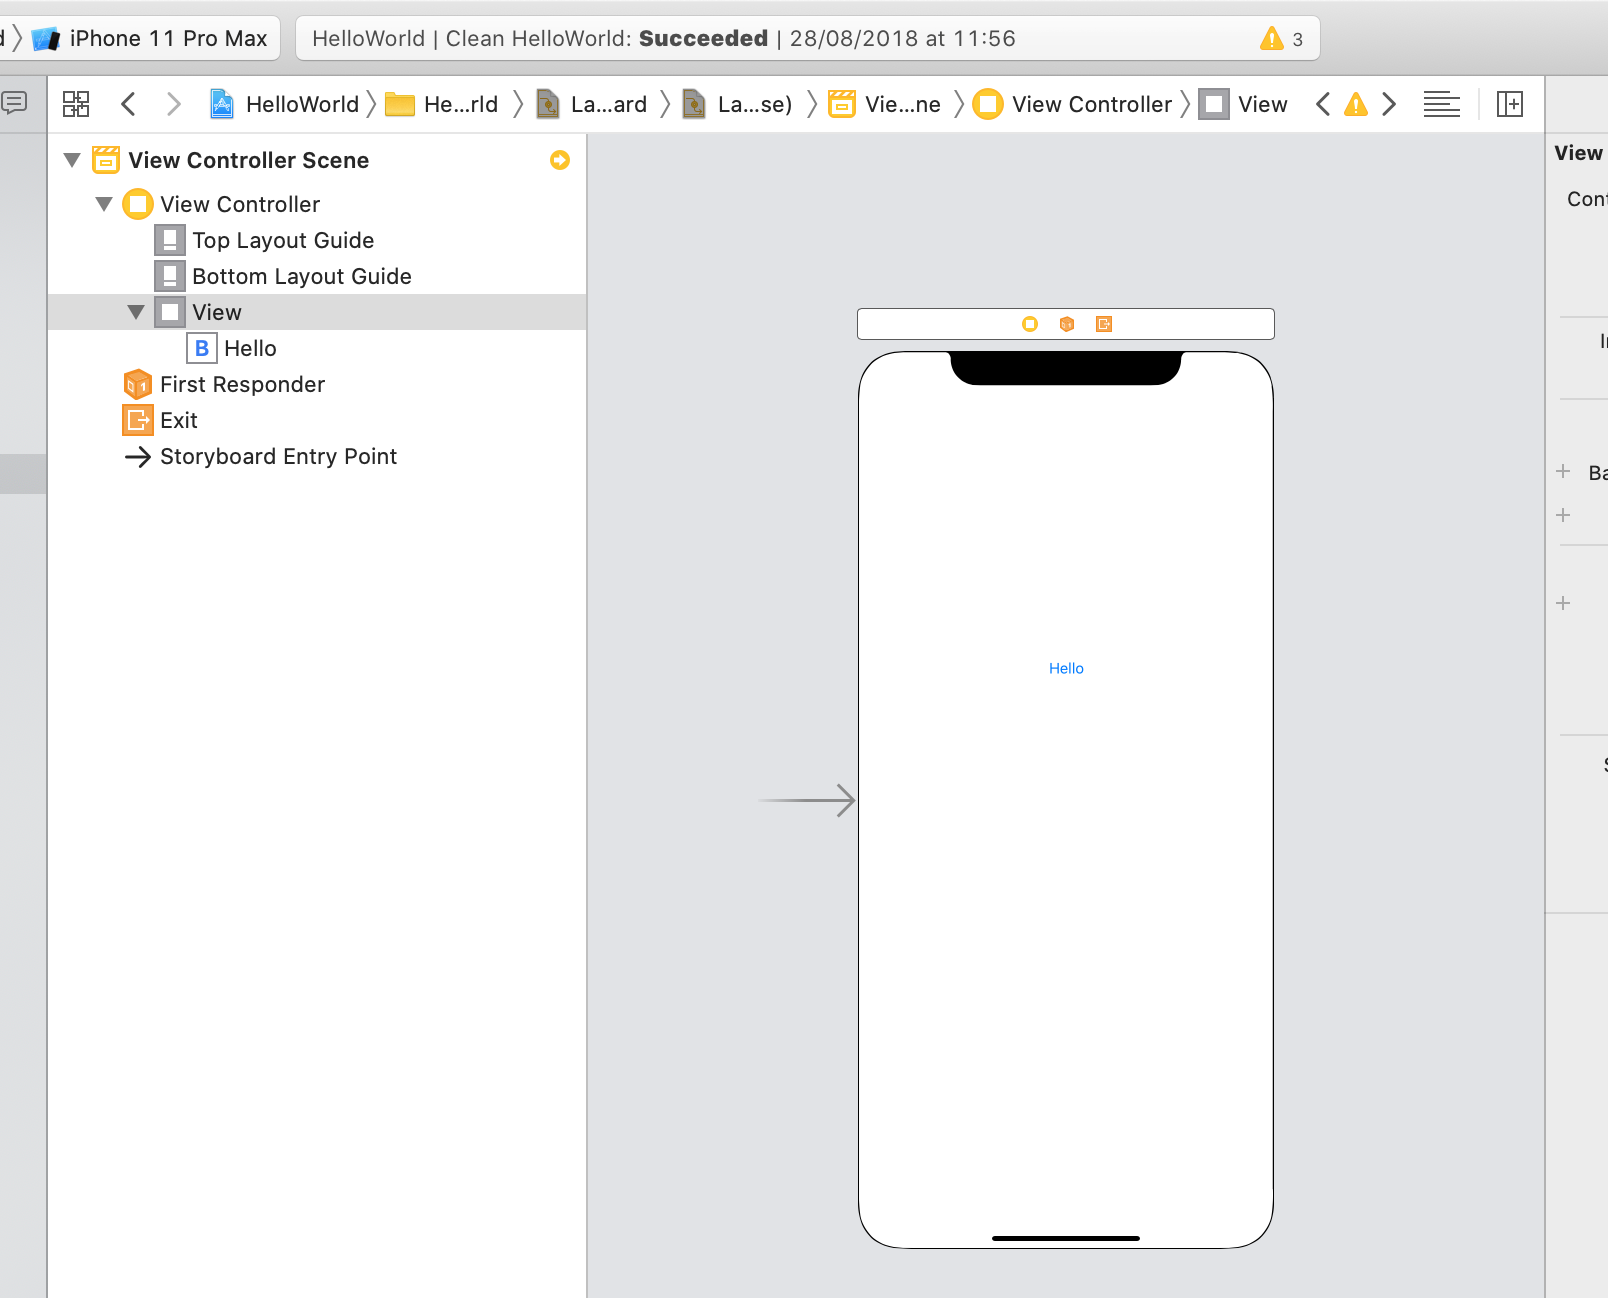
\includegraphics[width=0.8\textwidth]{chapters/06-appdev/img/xcode-interface.png}
  \caption{Construirea vizuală a interfeței unei aplicații într-un IDE}
  \label{fig:appdev:gui-interface}
\end{figure}

Un alt avantaj important al mediilor de dezvoltare integrate sunt metodele
avansate de a depana programele. Folosind sistemul de depanare integrat în IDE,
putem configura puncte în care să oprim execuția programului, după care putem
inspecta valoarea curentă a variabilelor folosite sau valorile întoarse de
funcții. Mai mult, putem chiar modifica valorile unor variabile pentru a
influența execuția programului.

În general, pentru fiecare limbaj de programare ales, avem un IDE adaptat
acestuia. Există totuși și destul de multe IDE-uri ce suportă mai multe limbaje.
Se recomandă folosirea unui IDE dedicat limbajului de programare folosit, dacă
acesta există, pentru că ne ușurează mult munca. Un IDE ne permite să ne
concentrăm pe scrierea codului, fără a ne consuma timp cu a rula comenzi pentru
compilarea, rularea sau depanarea acestuia.

Mai departe vom menționa câteva medii de dezvoltare importante pentru cele mai
folosite limbaje de programare.

\subsubsection{Microsoft Visual Studio și MonoDevelop}
\label{sec:appdev:dev:ide:mono}

Microsoft Visual Studio este editorul dedicat dezvoltării în C/C++ și C\#.
Pentru că este suportat doar pe sisteme Windows sau macOS, pentru sisteme Linux
recomandăm folosirea IDE-ului MonoDevelop. MonoDevelop este open source, dar
este susținut de Microsoft, împreună cu Microsoft Visual Studio.

\subsubsection{Eclipse}
\label{sec:appdev:dev:ide:eclipse}

Eclipse este unul din IDE-urile cele mai folosite pentru dezvoltarea de
aplicații Java. Înainte de apariția Android Studio, era folosit chiar pentru
dezvoltarea de aplicații Android, prin instalarea unei extensii.

\subsubsection{NetBeans}
\label{sec:appdev:dev:ide:netbeans}

NeatBeans e un IDE cu sursă deschisă specializat pentru limbajul Java. El oferă
o modalitate ușoară de a crea interfețe grafice pentru aplicații Java, împreună
cu editorul pentru dezvoltarea programelor.

\subsubsection{Xcode}
\label{sec:appdev:dev:ide:xcode}

Xcode este IDE-ul dezvoltat de Apple pentru crearea în principal de aplicații
pentru iOS și macOS. Este adaptat pentru C, Objective-C și Swift. Objective-C e
un limbaj de programare ce extinde limbajului C, folosit pentru dezvoltarea de
aplicații iOS și macOS. Swift este succesorul limbajului Objective-C.

O caracteristică importantă a Xcode este editorul de interfețe grafice integrat
(storyboardul), care permite generarea vizuală a interfețelor grafice și
conectarea mai multor ferestre fără necesitatea de a scrie cod.

În ceea ce privește editorul pentru scrierea codului sursă, oricare din
editoarele descrise mai sus suportă un număr mare de limbaje de programare și
este adaptat pentru acestea. Recomandarea noastră este să încercați mai multe
editoare și să alegeți pe cel pe care îl considerați cel mai comod în folosire,
iar pentru limbajele de programare care au un IDE dedicat, se recomandă
folosirea IDE-ului.

\subsection{Biblioteci și framework-uri}
\label{sec:appdev:dev:libs}

Un alt aspect de care trebuie să ținem cont în dezvoltarea programelor este
folosirea bibliotecilor și a framework-urilor.

Bibliotecile sunt colecții de resurse pe care le integrăm în aplicațiile noastre
pentru a ne ușura procesul de dezvoltare. De exemplu, dacă dorim să dezvoltăm o
aplicație Python care face cereri HTTP \abbrev{HTTP}{Hypertex Transfer
Protocol}, vom folosi biblioteca \textit{requests} care expune funcția
\textit{get()} pentru a face o cerere. Fără a folosi biblioteca, ar trebui să
scriem noi tot codul care se conectează la un server, generează pachetul pentru
cerere, îl trimite, apoi preia și interpretează răspunsul.

O unealtă asemănătoare bibliotecilor sunt framework-urile. Și acestea sunt
unelte care ușurează procesul de dezvoltare, dar ele oferă un schelet pe care
aplicația îl urmează pentru a beneficia de proprietățile framework-ului. Practic
putem să ne gândim că biblioteca e un modul care odată integrat în aplicație
aduce funcții sau constante noi pe care le putem folosi când e cazul, în timp ce
framework-ul impune anumite funcții sau elemente ce trebuie implementate în
aplicație și aplicația trebuie să se muleze după acea structură.

Pentru a putea integra biblioteci și framework-uri în aplicațiile pe care le
dezvoltăm, acestea trebuie să existe pe sistemul pe care lucrăm. Vom vedea mai
departe, că de multe ori fiecare platformă de dezvoltare specifică unui limbaj
vine cu propriul sistem de instalare a acestor module.

\subsection{Rularea programului}
\label{sec:appdev:dev:run}

Odată ce am scris codul sursă și am instalat bibliotecile sau framework-urile
folosite, pasul final este să rulăm programul. Complexitatea acestui pas depinde
de complexitatea programului obținut. Pentru un program simplu, cu un fișier
care conține codul sursă și care nu folosește nicio bibliotecă, în general, este
suficient să specificăm fișierul sursă și compilatorul sau interpretorul se
ocupă de restul procesului. \labelindexref{Listing}{lst:appdev:simple-compile} conține comanda de compilare și de rulare a unui program simplu.

\begin{screen}[caption={Compilarea și rularea unui program simplu},label={lst:appdev:simple-compile}]
student@uso:~$ gcc main.c -o main
student@uso:~$ ./main
\end{screen}

În cazul unui program complex care conține mai multe fișiere, vom rula mai multe comenzi, ca în \labelindexref{Listing}{lst:appdev:multiple-compile}. Linia 1 și linia 2 conțin comenzi de compilare, linia 3 este comanda de linking, iar linia 4 este comanda de rulare.

\begin{screen}[caption={Compilarea și rularea unui program din mai multe surse},label={lst:appdev:multiple-compile}]
student@uso:~$ gcc -c utils.c
student@uso:~$ gcc -c main.c
student@uso:~$ gcc utils.o main.o -o main
student@uso:~$ ./main
\end{screen}

\subsection{Automatizarea procesului de dezvoltare}
\label{sec:appdev:automation}

Cum am observat mai sus, pentru aplicații complexe, compilarea sau rularea
acestora constă în rularea unei secvențe de comenzi. Toate aceste comenzi
trebuie rulate indiferent dacă se aduc modificări majore programului, sau dacă
se schimbă doar o linie de cod. Astfel, nu e greu să ne dăm seama că avem nevoie
de o modalitate de a automatiza acțiunile necesare compilării și rulării
codului, astfel încât să rulăm o comandă simplă care să \textit{se ocupe de
tot}. Practic, putem să ne gândim că fișierele care alcătuiesc programul pe
care l-am dezvoltat sunt ingredientele necesare pentru o prăjitură, iar
prăjitura este executabilul sau chiar rezultatul rulării programului. Astfel,
similar unei rețete care descrie pașii necesari pentru a obține prăjitura, vom
scrie un fișier care conține pașii necesari obținerii rezultatului programului,
iar utilitarul în cauză este bucătarul care urmează rețeta.

Unele dintre utilitarele cele mai folosite pentru automatizarea acestor taskuri
sunt Make, Grunt, Gulp.

\section{Medii de dezvoltare}
\label{sec:appdev:dev-env}

Pentru fiecare limbaj de programare folosit avem nevoie de mediul de dezvoltare aferent (aplicații,
biblioteci, compilator și/sau interpretor), pentru a putea
rula aplicațiile pe care le scriem. Bineînțeles că putem scrie codul sursă în
orice editor, fără a folosi nici un alt program adiacent, dar am obține un fișier
cu instrucțiuni inutil, pe care nu îl putem compila sau interpreta. De aceea, în
primul rând, în funcție de tipul limbajului, avem nevoie de un compilator sau un
interpretor, care să ne permită acest lucru.

Pe lângă compilator sau interpretor, pentru folosirea unui limbaj de programare
avem nevoie să instalăm bibliotecile folosite.

Mai departe vom analiza particularități în instalarea compilatorului sau a
interpretorului pentru mai multe limbaje de programare.

\subsection{C / C++}
\label{sec:appdev:dev-env:c}

Pentru limbajul C, compilatorul cel mai cunoscut este GCC \abbrev{GCC}{GNU
Compiler Collection} (\textit{GNU Compiler Collection}). Conceput inițial pentru a
compila limbajul C, în momentul de față GCC a fost extins pentru a suporta
compilarea și a altor limbaje, cum ar fi C++ sau Java.

Pentru sistemele derivate din Debian, există un pacet special numit
\textit{build-essential}, instalabil folosind comanda:

\begin{screen}
student@uso:~$ sudo apt install build-essential
\end{screen}

Pentru sistemele derivate din Redat, precum Fedora, CentOS etc. trebuie
instalate pachetele separat folosind comanda:

\begin{screen}
student@uso:~$ sudo dnf install make gcc g++
\end{screen}

Toate aceste pachete vor instala și limbajul C++.

GCC poate fi instalat și pe sisteme Windows, prin intermediul unei aplicații
care care simulează un sistem Unix (Cygwin, MinGW etc.).

Pentru sisteme Windows, compilatorul de baza este integrat în aplicația
Microsoft Visual C++. Microsoft Visual C++ este un ecosistem de programare și
constă într-un editor cu funcții avansate (sugestii de completare a codului,
sugestii de posibile erori etc.) împreună cu compilatorul de C și C++ și se
recomandă folosirea acestuia pentru dezvoltarea de programe C.

Pentru C++ se poate folosi aceeași colecție de compilatoare ca pentru limbajul
C, adică GCC. Cum am menționat mai sus, în momentul de față GCC suportă
compilarea limbajului C++.

La folosirea gcc, sistemul analizează fișierele de intrare și hotărăște dacă
limbajul compilat este C sau C++. Pentru a eficientiza procesul, se poate folosi
direct g++, adică compilatorul de C++ integrat în gcc, ca în \labelindexref{Listing}{lst:appdev:simple-cpp}.

\begin{screen}[caption={Exemplu compilare si rulare C++},label={lst:appdev:simple-cpp}]
student@uso:~$ g++ main.cpp -o main
student@uso:~$ ./main
\end{screen}

De asemenea, pentru sisteme Windows mediul de dezvoltare recomandat rămâne
același. Microsoft Visual C++ este recomandat și pentru dezvoltarea de aplicații
C++.

\subsubsection{Dezvoltarea în C/C++}
\label{sec:appdev:dev-env:c-dev}

Cum mai menționat anterior, compilatorul cel mai folosit pentru C și C++ este
gcc/g++. Pentru folosirea compilatorului este suficient să rulăm comanda
\cmd{gcc} cu parametrii aferenți.

În procesul de compilare codul sursă este prelucrat și trece prin mai multe
etape intermediare:

\begin{enumerate}
	\item preprocesare: se înlocuiesc macro-uri, se numerotează fiecare
		linie de cod; rezultatul e un fișier cu extensia \textbf{.i}
	\item compilare: codul sursă este transformat în cod în limbaj de
		asamblare; rezultatul e un fișier cu extensia \textbf{.s}
	\item asamblare: codul în limbaj de asamblare este transformat în cod
		mașină; rezultatul e un fișier cu extensia \textbf{.o}
	\item link-editare: se fac legăturile către fișiere externe care conțin
		simboluri sau funcții apelate din fișierul sursă; dacă avem o
		funcție definită într-un fișier și folosită în altul,
		implementarea funcției trebuie legată de apelul ei;
\end{enumerate}

La simpla rulare a comenzii \cmd{gcc}, se trece prin toate etapele menționate.
De exemplu, pentru un program C simplu (\texttt{main.c} fără nicio bibliotecă) vom rula comenzile indicate în \labelindexref{Listing}{lst:appdev:simple-compile}.

În schimb, pentru programe mai complexe, alcătuite din mai multe fișiere, e
necesar să generăm fișierul obiect aferent fiecărui fișier sursă și apoi sa le
link-edităm pentru a obține executabilul final, așa cum am indicat în \labelindexref{Listing}{lst:appdev:multiple-compile}.

\subsubsection{Automatizarea compilării în C/C++}
\label{sec:appdev:dev-env:c-dev}

Cum am menționat mai devreme, este obositor să rulăm toate comenzile de mai sus
pentru fiecare modificare adusă în codul sursă. De aceea există posibilitatea de
a crea un fișier care conține toate aceste comenzi și care le poate rula pe
toate printr-un singur apel.

Utilitarul de automatizare cel mai folosit pentru aplicațiile C/C++ este utilitarul Make.
Pentru a folosi Make e suficient să creăm un fișier cu numele \file{Makefile} în
structura programului nostru. La rularea comenzii \cmd{make}, utilitarul găsește
acel fișier și execută instrucțiunile descrise.

Un fișier \file{Makefile} urmează formatul din \labelindexref{Listing}{lst:appdev:makefile-format}.

\begin{screen}[caption={Formatul unui fișier Maefile},label={lst:appdev:makefile-format}]
regula: dependente
<TAB> comanda
\end{screen}

Fișierul poate să conțină mai multe astfel de linii, precum fișierul \file{Makefile} din \labelindexref{Listing}{lst:appdev:makefile}.

\begin{screen}[caption={Exemplu Makefile},label={lst:appdev:makefile}]
build: utils.o hello.o help.o
       gcc utils.o help.o hello.o -o hello

all:
       gcc simple_hello.c -o simple

utils.o: utils.c
       gcc -c utils.c

hello.o: hello.c
       gcc -c hello.c

help.o: help.c
       gcc -c help.c

clean:
       rm -f *.o hello
\end{screen}

Regula reprezintă numele unei instrucțiuni. La simpla rulare a comenzii \cmd{make}
prima regulă din fișier este cea care va fi executată. În schimb, dacă vom scrie
\cmd{make clean}, se va executa comanda aferentă regulii \texttt{clean}.

Dependențele sunt fișiere și/sau reguli necesare pentru a putea rula o comandă.
Practic, la rularea unei comenzi se verifică dacă fișierul din dependență există.
Dacă acesta există, putem rula comanda, dacă nu, se caută o altă regulă cu acel
nume și se va rula acea comandă (dacă dependențele ei sunt îndeplinite, dacă nu,
se continuă lanțul de dependențe). Bineînțeles, sunt cazuri în care dependențele
pot să lipsească.

Acum să luăm cazul programului dezvoltat mai sus, care depinde de mai multe
fișiere și să presupunem că am schimbat o linie într-un fișier. La rularea
comenzii \cmd{make}, toate fișierele ar fi refăcute, ceea ce nu este eficient. De
aceea, \cmd{make} ține cont de încă un aspect la verificarea dependențelor. Dacă
dependența (fișierul) există, \cmd{make} va urmări lanțul de dependențe până ajunge la
fișierele de baza ale acesteia. Dacă fișierele au fost modificate după ce
dependența a fost creată, aceasta va fi regenerată, în caz contrar nu se va
regenera dependența.

\subsection{Java}
\label{sec:appdev:dev-env:java}

Fiind un limbaj hibrid, pentru Java sistemul de execuție a codului sursă este
mai complex. Cum am menționat mai sus, în general limbajele hibride trec
printr-o etapă de compilare în urma căreia rezultă un fișier bytecode, iar apoi
acel cod este interpretat.

Pentru majoritatea limbajelor hibride (Python, JavaScript) există un sistem care
conține atât compilatorul de bytecode cât și interpretorul, sau mașina virtuală.
Pentru Java, cele două elemente sunt separate clar, avem compilatorul care
generează codul sursă în bytecode și mașina virtuală ce execută fișierele
bytecode. Cele două se instalează separat, ca două aplicații diferite și
independente. Astfel, putem avea un sistem care doar generează fișierele
bytecode și un alt sistem care le execută.

În ceea ce privește platformele pentru a compila și a rula Java, putem alege
între două platforme principale: OracleJDK sau OpenJDK. Cum sugerează și numele,
OracleJDK este dezvoltată de Oracle, în timp ce OpenJDK este o platformă open
source și este special concepută pentru sisteme Unix. Pe lângă JDK (Java
Development Kit), putem instala OracleJRE sau OpenJRE (Java Runtime
Environment).

În timp ce JDK este sistemul complet ce compilează și execută aplicații Java,
JRE este doar mașina virtuală care rulează bytecode-ul generat de către
compilator. Ea este inclusă în JDK, dar poate fi instalată și separat. Astfel,
putem avea sisteme care doar rulează aplicații Java și care necesită bytecode-ul
generat de JDK.

Pe sisteme Linux OpenJDK este într-un pachet cu numele de forma \texttt{openjdk-X-jdk}, unde \texttt{X} este numele versiunii. De exemplu, pe Ubuntu 18.04 pachetul este \texttt{openjdk-8-jdk}.

Pentru sisteme care rulează Windows, se recomandă instalarea OracleJDK. Deși se
găsesc versiuni OpenJDK compatibile cu Windows, acestea nu sunt întreținute și
prezintă riscuri de securitate.

Pentru a instala OracleJDK pe un sistem Windows, accesați site-ul Oracle și
urmați instrucțiunile
(https://www.oracle.com/technetwork/java/javase/overview/install-windows-142126.html).

O particularitate a Java este aceea că bibliotecile sunt împachetate ca niște
arhive (jar - \textit{Java Archive}) care sunt incluse în aplicațiile pe care le
dezvoltăm. Fișierul \texttt{.jar} conține resurse diverse, de la definiții de clase la
imagini sau alte fișiere multimedia. Fiecare astfel de arhivă poate conține un
fișier manifest ce oferă informații despre pachet și despre utilizarea sa.

\subsection{C\#}
\label{sec:appdev:dev-env:csharp}

Pentru C\# sistemul de execuție este .NET, dezvoltat de Microsoft. Așadar,
sistemele cu Windows au deja sistemul instalat.

Pentru sisteme Unix, se recomanda folosirea Mono, cu ajutorul pachetului \texttt{mono-devel}. Mono este platforma
open-source pentru C\#, susținută tot de Microsoft.

Pentru aplicațiile dezvoltate în C\# putem folosi fie Mono, fie .NET. Indiferent
de platforma folosită, pentru a putea instala biblioteci putem folosi utilitarul
NuGet, dezvoltat de Microsoft.

La fel ca în Java, în C\# bibliotecile sunt similare unei arhive.

\subsection{Python}
\label{sec:appdev:dev-env:python}

La fel ca Java, Python e un limbaj de programare hibrid. Diferența între cele
două este că pentru Python nu se diferențiază compilatorul de mașina virtuală,
cele două sunt integrate.

Pentru a folosi Python pe un sistem Unix este suficient să instalăm pachetul \texttt{python}.

Pentru sistemele Windows, site-ul \textit{python.org} ne oferă resursele
necesare pentru instalare.

La instalarea interpretorului de Python este foarte importantă versiunea
acestuia. Putem alege între Python2 sau Python3, cele două fiind diferite.
Python 3.0 a fost lansat în anul 2008 și prezintă o sintaxă diferită de Python
2. De aceea este important să instalăm un interpretor potrivit pentru versiunea
Python pe care o folosim la dezvoltarea aplicațiilor.

Se recomandă folosirea Python3 deoarece Python2 nu mai este adus la zi.

Când vine vorba de dezvoltarea aplicațiilor folosind Python, abordarea e puțin
diferită de C, pentru că Python e un limbaj interpretat. Drept urmare, pentru a
putea rula programul pe care îl scriem, va trebui să rulăm interpretorul și să
îi spunem acestuia care e programul pe care dorim să îl interpreteze.

Pentru că în general vom lucra la proiecte complexe, care conțin mai multe
fișiere, similar cu programele din C, în Python vom avea un fișier de bază care
depinde de celelalte fișiere. Astfel, pentru a rula aplicația e suficient să
specificăm fișierul de pornire, ca în \labelindexref{Listing}{lst:appdev:python-example}.

\begin{screen}[caption={Exemplu rulare Python},label={lst:appdev:python-example}]
student@uso:~$ python main.py
\end{screen}

Cum am menționat mai sus, Python oferă un număr mare de biblioteci și
framework-uri care pot fi integrate în programele pe care le dezvoltăm. Pentru a
putea folosi o bibliotecă, aceasta trebuie să existe pe sistemul care rulează
programul. Pentru instalarea unei biblioteci, folosim utilitarul \cmd{pip}, așa cum am precizat în \labelindexref{Secțiunea}{sec:package:specific}.

\subsection{Node.js}
\label{sec:appdev:dev-env:js}

Când menționăm Node.js, ne referim deja la mediul de dezvoltare al aplicațiilor
JavaScript.

JavaScript este un limbaj folosit pentru aplicații web, iar interpretoarele de
JavaScript sunt integrate în browsere. De aceea a apărut Node.js, care e o
platformă ce permite executarea codului JavaScript în afară browserului. Unul
din interpretoarele de JavaScript este V8, dezvoltat de Google și integrat în
Google Chrome. Node.js integrează acest interpretor.

Pentru a instala Node.js pe sisteme Linux, recomandăm folosirea instanței Snap ca în \labelindexref{Listing}{lst:appdev:install-nodejs}.
Platforma se poate instala și instalând pachetul \texttt{nodejs} în mod clasic, dar se va descărca o versiune foarte veche a platformei.

\begin{screen}[caption={Instalare Node.js},label={lst:appdev:install-nodejs}]
student@uso:~$ sudo snap install --classic node
node (12/stable) 12.18.4 from NodeSource, Inc. (nodesource) installed

student@uso:~$ node
Welcome to Node.js v12.18.4.
Type ".help" for more information.
>
\end{screen}

Pentru instalarea pe sisteme ce rulează Windows, se recomandă descărcarea
kitului de instalare de pe site-ul Node.js.

În general, dacă alegem să dezvoltăm o aplicație folosind Node.js, dorim să
dezvoltăm o aplicație web la care atât partea de server, cât și cea de client să
fie scrise folosind JavaScript. Pentru partea de server vom folosi Node.js
pentru a putea rula programul, în timp ce partea de client va fi interpretată în
browser.

Când dezvoltăm o aplicație în Node.js, aspectele de care trebuie să ținem cont
sunt similare cu cele care au legătură cu Python. Similar cu Python, pentru
rularea codului sursă scris avem nevoie de interpretorul necesar instalat.

Pentru a rula o aplicație Node.js folosim comanda:

\begin{screen}
student@uso:~$ node main.js
\end{screen}

Pentru manipularea modulelor externe se folosește utilitarul \cmd{npm}. Pentru
instalarea unei biblioteci comanda necesară este \cmd{npm install $<$biblioteca$>$}.

Cum am menționat mai sus, de cele mai multe ori, când folosim Node.js, vom crea
aplicații complexe, de cele mai multe ori, aplicații web. De aceea, după ce
scriem codul sursă vom dori să îl prelucrăm. De exemplu putem alege să minimizăm
codul, adică să restrângem tot codul într-un singur fișier, greu inteligibil
pentru dezvoltatori, pentru a ne asigura că nu poate fi ușor copiat. Pe lângă
asta, putem alege să trecem tot codul sursă printr-un utilitar care verifică
dacă există greșeli, cum ar fi nedeclararea unei variabile.

Pentru că sunt multe astfel de operații pe care vrem să le aplicăm codului sursă
înainte de a-l distribui, putem automatiza întregul proces. Unul din utilitarele
folosite la această automatizare este \cmd{grunt}. Putem să ne gândim la \cmd{grunt}
ca la un utilitar semănător cu Make, doar că operațiile pe care \cmd{grunt} le
efectuează implică preprocesarea codului sursă. Similar cu un fișier \file{Makefile}, pentru
\cmd{grunt}, vom crea un fișier numit \file{Gruntfile} care conține toate regulile, ca în \labelindexref{Listing}{lst:appdev:gruntfile}.

\begin{screen}[caption={Exemplu cod Gruntfile},label={lst:appdev:gruntfile}]
module.exports = function(grunt) {

 grunt.initConfig({
   jshint: {
     files: ['Gruntfile.js', 'src/**/*.js', 'test/**/*.js'],
     options: {
       globals: {
         jQuery: true
       }
     }
   },
   watch: {
     files: ['<%= jshint.files %>'],
     tasks: ['jshint']
   }
 });

 grunt.loadNpmTasks('grunt-contrib-jshint');
 grunt.loadNpmTasks('grunt-contrib-watch');

 grunt.registerTask('default', ['jshint']);

};
\end{screen}

\section{Depanarea programelor}
\label{sec:appdev:debug}

Pe măsură ce scriem tot mai multe programe, ne dăm seama că de cele mai multe
ori acestea nu funcționează cum ne dorim de la început. De multe ori se va
întâmpla ca programul rulat să arunce o eroare sau să nu obțină rezultatul
dorit. Deși am dori să putem spune că \textit{e vina calculatorului}, orice
eroare sau comportament eronat apare dacă noi nu am scris ceva bine în codul
sursă. Erorile pot să varieze de la un simbol uitat,
la accesări ilegale de memorie sau chiar erori în logica programului. Astfel, o
mare parte din timpul destinat dezvoltării aplicațiilor îl dedicăm depanării. De
aceea e de preferat să fim eficienți în descoperirea erorilor.

Am menționat mai sus că unul din aspectele importante ale unui IDE este
posibilitatea de a seta puncte de oprire în execuția programului. Astfel, odată
ce o linie de cod este executată, întregul proces se oprește și noi putem
monitoriza starea curentă. Adică putem vizualiza valorile pe care le au
variabilele sau adresele de memorie la care se găsesc, ca în \labelindexref{Figura}{fig:appdev:ide-debug}.

\begin{figure}[!htbp]
  \centering
  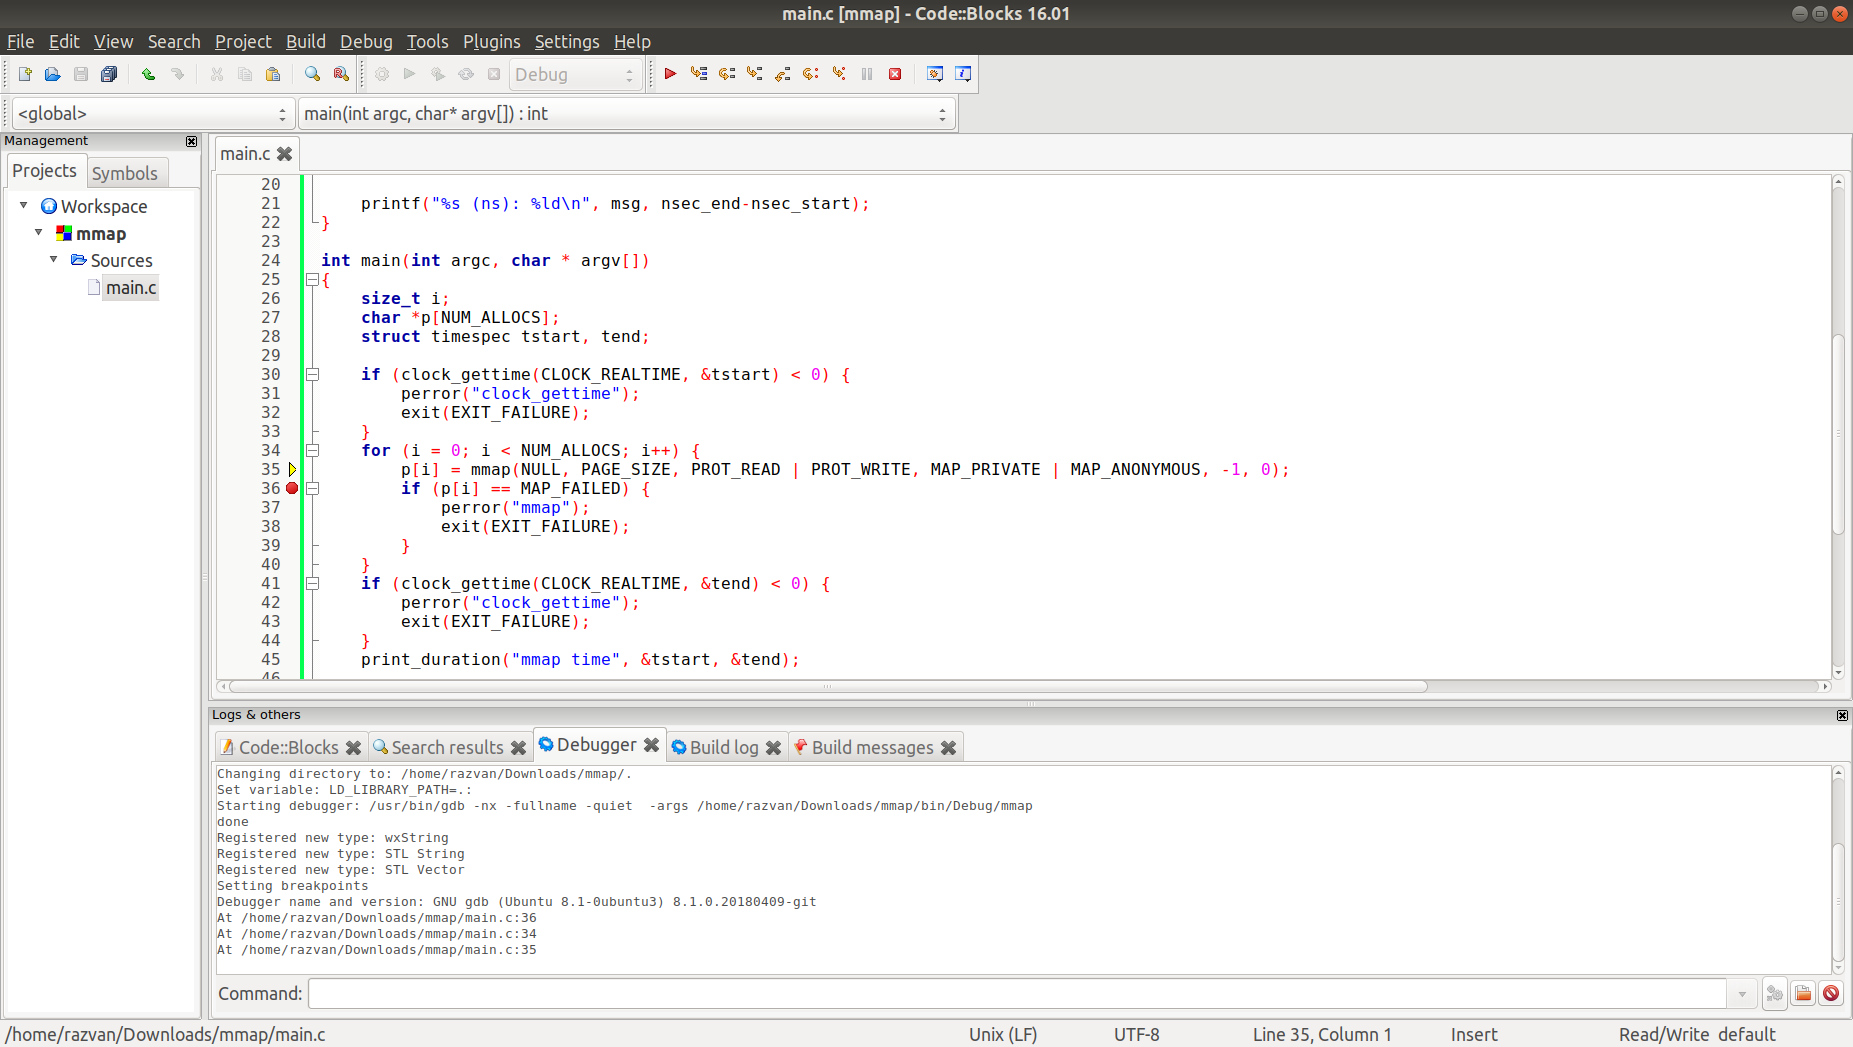
\includegraphics[width=\textwidth]{chapters/06-appdev/img/codeblocks-debug.png}
  \caption{Interfață de depanare într-un IDE (coblocks)}
  \label{fig:appdev:ide-debug}
\end{figure}

Unul dintre cele mai cunoscute utilitare pentru depanare este GDB. GDB oferă suport pentru
toate operațiile menționate mai sus și este compatibil cu toate sistemele de
operare existente.

Cea mai simplă metodă de a depana un program este să afișăm mesaje pe parcursul
execuției. Astfel putem vizualiza valorile variabilelor sau blocurile de cod
care se execută sau nu. Deși pare un mod primitiv de a face depanare, este cel
mai la îndemână.

De fiecare dată când ceva nu funcționează, se recomandă verificarea pas cu pas a
liniilor de cod și printarea rezultatului. De foarte multe ori eroarea se
observă prin afișarea variabilelor.

În plus, nu este o practică eficientă să scriem zeci de linii de cod fără a
testa. E recomandat să scriem în incremente mici și să ne asigurăm ca fiecare
bloc funcționează. Altfel, ne vom trezi puși în fața a zeci de linii de cod care
nu funcționează și va fi dificil să identificăm problema.

\section{Sisteme de management și versionare a codului sursă}
\label{sec:appdev-versioning}

De cele mai multe ori, vom lucra la proiecte complexe, în cadrul unei echipe.
Acest lucru înseamnă că vom avea multe fișiere cu cod sursă pe care le vom modifica în
paralel cu alte persoane. Drept urmare, avem nevoie de o modalitate de a împărți
proiectul într-un mod eficient. Deși la început acest lucru nu pare neapărat
dificil, pe măsură ce proiectul crește, este tot mai greu. Pe lângă partajarea
efectivă a întregii structuri a programului, avem nevoie de o modalitate de a
urmări modificările aduse și cine ce modificări a făcut. Să ne gândim la
situația în care suntem o echipă de 5 oameni și cineva face o modificare ce
rezultă într-un comportament defectuos al programului. Având în vedere că suntem
5 oameni care au adus simultan modificări codului sursă, va fi dificil să
identificăm eroarea. În cazul unui proiect avansat, problema e și mai mare.

De aceea metode precum \textit{folosim un director online comun sau chiar
trimitem sursele modificate prin email} nu sunt recomandate pentru a lucra în
echipă la un proiect și de aceea există sisteme dedicate partajării de cod
sursă. Un astfel de sistem este Git.

Git este un sistem de management și versionare a codului sursă care permite
partajarea unui proiect în cadrul unei echipe. Proiectul este stocat într-un
depozit (\textit{repository}). Repository-ul conține fișierele efective ale proiectului și
multe alte informații despre acesta. Folosind Git, fiecare persoană lucrează la
o versiune proprie a proiectului, pe care apoi o urcă online și este automat
integrată în proiect. Ceilalți colaboratori descarcă modificările aduse când
doresc. Sistemul urmărește modificările pe care fiecare persoană le aduce și la
orice moment putem descărca o versiune anterioară a codului sursă. Pentru a
realiza toate acestea avem la dispoziție următoarele operații de bază:

\begin{itemize}
  \item \cmd{clone}: se clonează întreg repository-ul pe sistemul local;
		practic se va crea un director care conține toate fișierele
		aferente programului, plus niște fișiere care stochează
		informații despre proiect (ex, cine a creat repository-ul, ce
		modificări au fost aduse etc. );
  \item \cmd{commit}: se salvează toate modificările aduse proiectului; starea
		actuală este salvată local; dacă modificările nu sunt publicate
		online, acestea nu sunt vizibile colaboratorilor;
  \item \cmd{push}: se publică modificările salvate prin commit; odată
		publicate aceste modificări, colaboratorii pot să vizualizeze
		cine le-a adus și pot să urmărească schimbările linie cu linie
  \item \cmd{pull}: se descarcă local ultimele modificări publicate de ceilalți
		colaboratori și se integrează în versiunea locală a proiectului.
\end{itemize}

\section{Licențe pentru programe}
\label{sec:appdev:license}

Un aspect important când vine vorba de dezvoltarea programelor este
licența acestuia.

Licența unui program oferă informații despre dreptul de folosire și distribuție
a programului.

De multe ori vom dori să publicăm programele pe care le dezvoltăm pentru a
permite altor persoane să le folosească sau chiar să le integreze în proiectele
proprii. Când facem acest lucru, este important să definim scopul aplicației pe
care o dezvoltăm și să îi atribuim o licență corespunzătoare. Astfel, cei care
vor folosi programul nostru vor ști ce pot și ce nu pot să facă cu el.

Pe de altă parte, în procesul de dezvoltare a unui program vom folosi un număr
semnificativ de biblioteci și framework-uri. Când facem acest lucru este foarte
important să verificăm licența fiecărui pachet extern pe care îl integrăm în
aplicația noastră. Licențele modulelor externe folosite pot influența folosirea
programului pe care îl dezvoltăm.

Acum că știm că e important să stabilim o licență pentru programele pe care le
dezvoltăm, întrebarea care urmează este, cum stabilim aceste reguli și cum
alegem licența potrivită. De foarte multe ori chiar licența unui modul extern
folosit poate dicta licența pe care trebuie să o atribuim programului nostru. Ca
să înțelegem mai bine ce caracteristici poate să aibă o licență, vom menționa
cele mai cunoscute și folosite licențe software.

\subsection{GNU GPL}
\label{sec:appdev-licensing-gpl}

GNU \abbrev{GNU}{GNU's Not Unix} GPL \abbrev{GNU GPL}{GNU General Public
License} este prescurtarea de la \textit{GNU General Public License} și de cele mai multe
ori ne referim la această licență drept GPL.

Un program însoțit de o licență GPL poate fi distribuit doar dacă sursa acestuia
este publică și programul poate fi integrat în orice alt program care este
public și nu are nicio restricție de folosire. Practic, orice program care
folosește un modul GPL trebuie să aibă la rândul lui licență GPL. În plus,
biblioteca integrată poate fi modificată

\subsection{GNU LGPL}
\label{sec:appdev-licensing-lgpl}

GNU LGPL \abbrev{GNU LGPL}{GNU Lesser General Public License} (simplu LGPL) este
o licență cu restricții mai reduse față de GNU GPL. Numele vine de la \textit{GNU
Lesser General Public License}. În cazul acestei licențe programul în cauză poate
fi integrat în alte programe care au orice altă licență. Singura restricție este
ca modulul LGPL folosit să fie făcut public în cadrul aplicației. De asemenea,
în cazul în care biblioteca LGPL este modificată și abia apoi integrată într-o
aplicație, biblioteca modificată trebuie publicată sub licență LGPL.

\subsection{MIT}
\label{sec:appdev-licensing-mit}

MIT \abbrev{MIT}{Massachusetts Institute of Technology} este o licență mai
permisivă față de GPL. Orice bibliotecă care are licența MIT poate fi integrată
în orice program și acesta poate fi distribuit, fără necesitatea de a face
programul public. Singura condiție este ca licența MIT să apară în programul
principal.

\section{Sumar}
\label{sec:appdev-summary}

Pe parcursul acestui capitol am prezentat principalele tipuri de limbaje de
programare: compilate, interpretate și hibride. Am discutat despre avantajele și
dezavantajele fiecăruia. De asemenea, am trecut în revistă principalele limbaje
de programare folosite din fiecare categorie, evidențiind unde se folosește
fiecare.

Sunt importante de reținut etapele dezvoltării unei aplicații. În primul rând,
trebuie să hotărâm ce aplicație dorim să realizăm, cine o va folosi și care va
fi mediul hardware și software în care va rula. Odată stabilite acestea, trebuie
să alegem limbajul potrivit, mediul de programare și să instalăm bibliotecile
necesare.

Următorul pas este scrierea codului sursă, compilarea acestuia și testarea lui.
Acest proces este repetat de foarte multe ori până la definitivarea aplicației.

Odată ce aplicația funcționează corespunzător, trebuie să îi adăugăm o licență
de distribuție și să facem un pachet de instalare.

Aplicația este gata de lansare.
